\documentclass{fcs}
\usepackage{bm}
\usepackage[utf8]{inputenc}
\usepackage{amssymb}
\setcounter{tocdepth}{3}
\usepackage{float}
\usepackage{caption}
\usepackage{graphicx}
\usepackage{subfigure}
\usepackage[ruled,vlined]{algorithm2e}
\graphicspath{{images/}}

\usepackage{multicol} % enable multicolumn
\usepackage[table]{xcolor}
\usepackage[]{booktabs}
\usepackage{hyperref}
\hypersetup{
    colorlinks=true,
    linkcolor=blue,
    filecolor=magenta,      
    urlcolor=blue,
}

% to typeset URLs, URIs, and DOIs
\usepackage{url}
\def\UrlFont{\rmfamily}

\newcommand{\keywords}[1]{\par\addvspace\baselineskip
\noindent\keywordname\enspace\ignorespaces#1}

\makeatletter
\newcommand{\printfnsymbol}[1]{%
  \textsuperscript{\@fnsymbol{#1}}%
}
\makeatother

%% Volumn number
\volumn{ }
%% DOI
\doi{ }
%% Types of papers, can be
%%   RESEARCH~ARTICLE
%%   REVIEW~ARTICLE
%%   EDITORIALS
\articletype{RESEARCH~ARTICLE}
%% Copyright notice
\copynote{{\copyright} Higher Education Press and Springer-Verlag Berlin Heidelberg 2012}
%% Time of receive and acceptance
\ratime{Received month dd, yyyy; accepted month dd, yyyy}
%% Email address of the corresponding author
\email{$fquiroga@lidi.info.unlp.edu.ar$}
%% Title
\title{$\bm{Recognizing~ Handshapes~ using~ Small~ Datasets}$}
%% Authors
\author{Ulises Jeremias Cornejo Fandos $^{1}$, Gastón Gustavo Rios $^{1,2}$, Franco Ronchetti $^{1,3}$, Facundo Quiroga \xff $^{1,4}$, Waldo Hasperué $^{1,5}$ and Laura Lanzarini $^{1}$}
%% Addresses of authors
\address{{1\quad Instituto de Investigación en Informática III-LIDI, Facultad de Informática, Universidad Nacional de La Plata}\\
{2\quad Becario doctoral - Universidad Nacional de La Plata }\\
{3\quad Investigador Asistente - Comisión de Investigaciones Científicas (CICPBA)}\\
{4\quad Becario postdoctoral - Universidad Nacional de La Plata}\\
{5\quad Investigador Asociado - Comisión de Investigaciones Científicas (CICPBA)}}

%% Running head
\markboth{Recognizing Handshapes using Small Datasets}{Recognizing Handshapes using Small Datasets}

\begin{document}
\maketitle
\setcounter{page}{1}

\begin{abstract}

\noindent The development of a sign language recognition model with high performance would be a great improvement in the communication with and within  deaf communities. The main issue preventing effective models lays on the low availability of labeled data which complicates the use of modern deep learning models of a big labeled data source. For this reason we compare a series of models and training procedures specially tailored for small datasets to improve the performance over previous state-of-the-art models. We trained DenseNet and few-shot Prototypical Network models with and without transfer learning, and also using Model-Agnostic Meta-Learning (MAML), a method specifically tailored to tackle few-shot learning. Our main findings indicate that DenseNet without transfer learning and Prototipical Networks with transfer learning provide the best results on most tasks. Using a meta-learning technique such as MAML does not seem to improve the performance of DenseNet w.r.t to traditional training. We also measure the effect of the training set size on the performance of the models, and found that, in general, prototypical networks are superior when using less than 30 samples.

\end{abstract}

\Keywords{sign language, handshape recognition, convolutional neural networks, densenet, prototypical networks, model-agnostic meta-learning, transfer learning, small datasets}


\section{Introduction}
\noindent Sign language is a system of communication that uses signs with the hands and other movements, including facial expressions and postures with the body to communicate meaning, commonly used by deaf people.

Sign Language Recognition is a field in the intersection of computer vision and language translation that seeks to create systems capable of translating videos of people speaking in sign language into text.

Sign language recognition presents an interesting challenge as the available data is limited compared to other problems for example speech recognition \cite{bragg2019}. The nature of the problem complicates the creation of new sign language datasets. Furthermore, merging datasets from different regions or countries is impossible since each sign language has its own syntax and semantic. Producing a model capable of recognizing sign language with high precision would improve the quality of life of many people since an automatic interpreter would facilitate communication between signers and non signers.

In this paper we address the low availability of data by implementing a variety of state-of-the-art convolutional neural network models and training techniques designed to tackle small labelled datasets. We compare two model architectures: Prototypical Network \cite{protonet} and DenseNet \cite{densenet}. We train these models with regular training and with Transfer Learning and Model Agnostic Meta Learning (MAML) \cite{DBLP:journals/corr/FinnAL17}.

DenseNet is a well known state-of-the-art model that has shown good performance for image classification even in cases where there is a low amount of labeled data\cite{densenet}. When the amount of available data is reduced even further, few-shot learning techniques are required. We chose Prototypical network as our specialized few-shot learning model. Prototypical networks are models based on metric learning, optimizing a distance function between classes in an embedded space to classify each sample.

In this work we propose to evaluate and compare new methods devoted to deal with small datasets in order to improve the current state-of-the-art in hand shape recognition for sign language.

Our approach consists of comparing different techniques for improving model performance in these conditions: prototypical networks for few shot learning,  transfer learning and model-agnostic meta-learning. We use the same data augmentation scheme for every experiment which consists of basic augmentation operators such as rotations, translations  and crops.

In the following subsection we summarize previous efforts on training CNN on handshape datasets. Section \ref{sec:datasets} describes the datasets and section \ref{sec:models} describes models and techniques we employed in our experiments, which are detailed along with results in Section \ref{sec:experiments}, and Section \ref{sec:conclusion} contains the conclusion of our work.

\subsection{Related Work}

Recent years have seen the rise in the use of deep learning models for sign language recognition, specifically the use of convolutional neural networks to extract image features or classify hand images. \cite{koller16}  trained a CNN to recognize handshapes  from the  RWTH handshape dataset,  which contains 3200 labeled samples and 50 different classes.  The model was based on a pre-trained network with a VGG architecture, and employed a semi-supervised scheme to take advantage of approximately  one million weakly labeled images, achieving an accuracy of 85.50\%. This constitutes the first attempt at adapting a model to overcome the low availability of labeled images for training. \cite{Ronchetti2016}  employed a radon transform as a feature for an ad hoc classifier that employed clustering as a quantization step and K nearest  neighbors  for the final classification. They tested the model on the LSA16 dataset, which contains only 800 examples, obtaining an accuracy of 92.3\%. \cite{quiroga2017study}  evaluated several CNNs on the LSA16 and RWTH datasets, including both vanilla and pre-trained models. The use of pretrained models helps to alleviate the lack of labeled data, since pretraining the convolutional filters establishes a prior that a classifier can exploit for handshape recognition. Their best models of an accuracy of 95.92\% for LSA16 and 82.88\%  for RWTH. \cite{ciarp2018} trained a simple neural network to classify a new dataset they created which we will call CIARP. CIARP contains 6000 examples and 10 classes, and the authores report an accuracy of 99.20\% with that model. \cite{tang2015real} train a CNN on a custom dataset with 36 classes, 8 subjects and 57000 sample images, obtaining an accuracy of 94.17\%. However, the samples correspond to video sequences and therefore are highly correlated;  while there are approximately 2000 images per class, there are only eight image sequences, one for each subject. Since each image sequence contains approximately 250 images  which are highly correlated, they only consider eight image per sequence per class. \cite{ameen2017fingerspelling} trained a simple CNN with only 6 layers using the ASL Finger spelling dataset, obtaining an accuracy of 80.34\%. The dataset consists of 60000 images of 25 different classes, but they were captured as videos so they are also highly correlated as in the previous case. \cite{barros14multichannel} employed the Jochen Triesch Database (JTD), which contains only 10 classes and  72 samples per class, as well as the NAO Camera Hand Posture Database, which contains 4 classes and 400 examples per class. They trained a simple CNN with a multichannel image containing the results of the Sobel operator as input, obtaining an F-score of 94\%  and  98\% in  each dataset perspective. \cite{alani2018peru} trained a deep CNN on the Hand Gesture Dataset LPD,  which contains 3250 images of only 6 classes, obtaining an accuracy of 99.73\%. \cite{cornejo2019hand} performed experiments with Wide-DenseNet and Prototypical Networks on the CIARP, LSA16 and RWTH datasets using vanilla models. In both cases, they also quantify the impact of data augmentation on accuracy. Their best models obtain an accuracy of 99.26\% on LSA16, 94.00\% on RWTH and 100.00\% on CIARP. This work is the third \cite{quiroga2017study,koller16:deephand} and last instance we found where a specific strategy was employed to alleviate the lack of data

This brief review confirms our previous statement that  while CNN are being consistently applied to handshape recognition tasks, most of these datasets are small and ad hoc, that is, recorded specifically for the purpose of testing a single model and not developed with the intent of providing a benchmark and complete training set for handshape recognition models. It is also worth noticing that some datasets are so small that it is very easy to obtain near-perfect performance with simple models. Also, many datasets are not readily available,  given that the authors have not published the data and do not provide any means of obtaining it.  

We note that the RWTH and LSA16 are both publicly available and current models have been shown to achieve less than perfect accuracy for them.  While the dataset in \cite{ciarp2018} (denoted CIARP in this paper) has been solved completely,  it is interesting and complementary because it targets general handshapes instead of those specific to sign language.


\section{Datasets}
\label{sec:datasets}
We selected three datasets, LSA16 \cite{Ronchetti2016}, RWTH-PHOENIX-Weather (RWTH) \cite{koller16:deephand} and CIARP \cite{ciarp2018}, because they contain images whose setting varies greatly, have been evaluated already, and possess different quantities of examples or distributions of samples per class.

\subsection{LSA16} LSA16 \cite{Ronchetti2016} contains images of 16 handshapes of the Argentinian Sign Language (LSA), each performed 5 times by 10 different subjects, for a total of 800 images of size 32x32. The subjects wore colored hand gloves and dark clothes on a white background. The dataset is balanced, with 50 images per class. There is only one hand in each image. The hands are centered and segmented from the background.

\subsection{RWTH} RWTH \cite{koller16:deephand} is composed of a selection of  han images of size 132x92 cropped from  videos of the sign language interpreters at the German public tv-station PHOENIX. There are a total of 45 different hand signs. The interpreters wore dark clothes in front of an artificial grey background. Many images posses significant movement blur, others contain both hands of the interpreter and hands are not always perfectly centered.

The dataset is highly imbalanced with some classes having just 1 sample while others have as many as 529 samples. We removed classes that had less than 40 samples following \cite{quiroga2017study}, to guarantee a minimum amount of images per class for the networks to learn.

\subsection{CIARP} CIARP \cite{ciarp2018} contains 6000 images of size 38x38 acquired by a single color camera. The images were manually labeled and correspond to 10 classes of hand gestures. The hands are centered and were segmented from the background, which was replaced by black pixels. The small size of the images and low amount of classes give this dataset lower complexity compared to LSA16 and RWTH. The classes in the data set correspond to handshapes which are not based on sign language, but are similar enough  so that the comparison remains valid.

\begin{figure}[!ht]
    \centering
    \begin{tabular}{ccccc}
        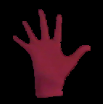
\includegraphics[height=4em,width=13.5mm]{datasets/lsa161.png} &
        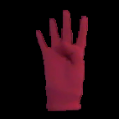
\includegraphics[height=4em,width=13.5mm]{datasets/lsa162.png} &
        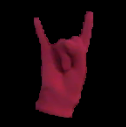
\includegraphics[height=4em,width=13.5mm]{datasets/lsa163.png} &
        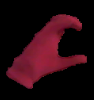
\includegraphics[height=4em,width=13.5mm]{datasets/lsa164.png} &
        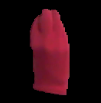
\includegraphics[height=4em,width=13.5mm]{datasets/lsa165.png} \\
        \multicolumn{5}{c}{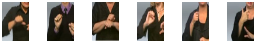
\includegraphics[width=23em]{datasets/rwth2.png}} \\
        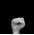
\includegraphics[height=4em,width=13.5mm]{datasets/ciarp1.png} &
        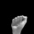
\includegraphics[height=4em,width=13.5mm]{datasets/ciarp5.png} &
        
\includegraphics[height=4em,width=13.5mm]{datasets/ciarp3.png} &
        
\includegraphics[height=4.01em,width=13.5mm]{datasets/ciarp4.png} &
        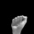
\includegraphics[height=4em,width=13.5mm]{datasets/ciarp5.png} \\
    \end{tabular}
    \caption{Sample images from the LSA16 (first row), RWTH-PHOENIX-Weather (second row) and CIARP (third row) datasets.}
    \label{fig:datasets}
\end{figure}


\section{Architectures and Techniques}
\label{sec:models}
We compared two different base classification models to analyze their ability to learn from these small handshape datasets; Prototypical Networks \cite{protonet} and DenseNet \cite{densenet}. Prototypical Networks is a model that was designed explicitly to deal with small sample sizes. On the other hand, DenseNet is currently a state of the art model in image classification with convolutional neural networks, and while it has not been explicitly designed for small datasets, it has shown exceptional performance in many different tasks. 

In the case of DenseNet, we also experiment using Model-Agnostic Meta-Learning (MAML) \cite{DBLP:journals/corr/FinnAL17} and Transfer Learning \cite{tan2018} training techniques, in addition to the traditional training process. 

Transfer Learning is a well known technique to jump-start the training of neural networks for a problem A using datasets from a similar problem B. The weights of a network trained on B are used as initial weights in the training of the network for A. Retraining the network for A is called finetuning, and may retrain only a subset of the weights of the network. However, it still may require large amounts of data for the finetuning phase.

Finally, MAML is a meta-learning technique for few-shot learning, that involves learning subtasks. In this context, each subtask corresponds

In the following subsections we describe in more detail each of these models.

\subsubsection{Wide-DenseNet}

We selected a DenseNet based architecture as it is a state of the art model in many domains and can handle small datasets with low error rate \cite{pmlr-v80-pham18a}.

DenseNet \cite{densenet} works by concatenating the feature-maps of a convolutional block to the feature-maps of all the previous convolutional blocks and using the resulting set of feature-maps as input for the next convolutional block. In this way, each convolutional block receives all the collective knowledge of the previous layers maintaining the global state of the network which can be accessed.

We employed a variation on DenseNet called Wide-DenseNet which follows the strategy used by wide residual networks \cite{He2015DeepRL}. Wide-DenseNet consists on decreasing the depth of the network and increasing the width of the layers. This way the model can be trained faster by optimizing feature reuse and obtain higher accuracy.

Additionally, we use Squeeze and Excitation blocks (SE blocks) \cite{Hu2017SqueezeandExcitationN} to improve the performance of the DenseNet model. Convolutional networks construct informative features by fusion both spatial and chanel-wise information within local receptive fields at each layer. SE blocks focus on  channel-wise information, improving the quality of the representations produced by the network by modeling the interdependency between channels to perform feature recalibration. SE blocks can be included in any model that uses convolutional layers to improve its performance at low computational cost. We use SE blocks between dense and transition blocks, see figure \ref{fig:densenet}.

\begin{figure*}[!ht]
    \centerline{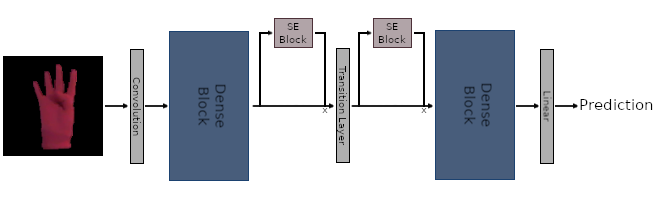
\includegraphics[width=0.85\textwidth]{images/background/densenet.png}}
    \caption{DenseNet using 2 dense blocks and SE blocks.}
    \label{fig:densenet}
\end{figure*}

\subsubsection{Transfer Learning} \label{models:tl}

Gathering new training data for deep neural networks can be an expensive and time consuming task. Transfer learning provides a way to utilize already available data from a source domain and transfer the acquired knowledge from this source domain to a target domain. By doing transfer learning we can obtain much better initializations of the parameters of the model before training in the target domain. 

In the past, transfer learning has been used for handshapes, sign language and gesture recognition \cite{farhadi2007}\cite{quiroga2017study}\cite{allard2017} demonstrating the advantages of this technique. 

In this work,  we are doing Network-based \cite{tan2018} transfer learning. In this type of transfer learning a part of the network pretrained on the source domain is reused for the training in the target domain. The objective is for the neural network to acquire abstract information from the source domain and transfer this knowledge to the target task.

To obtain a good performance from transfer learning it is commonly needed for the source dataset to be larger than the target dataset. Since the information extracted from the target dataset has a higher value than the information from the source dataset, the data from the target dataset will be more helpful in fitting the target task. In addition to this, it is important for the source domain to be well related to the target domain. If the relation between both domains differ too much it is possible to get a negative transfer which can diminish the performance obtained by using transfer learning to the point of obtaining less performance by applying it \cite{weiss2016}.

\subsubsection{Model-Agnostic Meta-Learning} \label{sec:models:maml}

Like Prototypical Networks, Model-Agnostic Meta-Learning (MAML) \cite{DBLP:journals/corr/FinnAL17} is a technique designed to tackle the problem of few-shot learning. MAML learns how to improve a model so that it can learn a new task in only a few steps by training on many different tasks, commonly phrased as learning to learn. MAML does this by learning over multiple tasks and updating the parameters of the models based on the improvement obtained after training on each task.

More formally, given a set of tasks $T$ each consisting of a loss function $L$ and a set of elements with their corresponding labels. MAML requires a distribution over tasks $p(T)$ that we want to adapt to. Given those distributions, we proceed with the next two steps, task training and meta training. In the task training we sample $K$ tasks. For each task $T_i$, the model is trained on a set of elements extracted from the task distribution using the loss function $L_i$ belonging to $T_i$. With the updated parameters the model is then tested on new data from $T_i$. Once tested on each task the loss obtained from these tests will be added and utilized as loss for the initial model on the meta training obtaining a new initial model with better initial parameters that will grant a bigger improvement for each task on fewer steps.

We made some modifications on the original MAML to work with bigger datasets in a supervised way. Each task $T_i$ is split in 2 subsets, a training subset $Tt$ and a meta training subset $Tm$. The subsets are composed of datasets $D={x,y}$ where $x$ is an image and $y$ the label of that image. Each subset has an equal size $b$ and its labels are mirrored $y\in Tt \iff y\in Tm$. Each dataset with size $n$ has $n/2b$ tasks $T$. We consider our model as a function $f_\theta$ with parameters $\theta$. In each training iteration $\theta$ will change to $\theta'$. Each iterations consists of 2 steps, a training and a meta training step. In the training step we start by storing the value of $\theta$ in $\theta'$, then $\theta$ is updated to fit $Tt_i$. In the meta training step the new $\theta$ is used to calculate the gradients with $Tm_i$ : $\nabla L_i(  f_\theta(Tm_i))$ and these gradients are applied to $\theta'$ finishing the iteration. 

\begin{algorithm}[!h]
\caption{Model-Agnostic Meta-Learning for Few-Shot Supervised Learning}
\SetAlgoLined
\KwIn{A set of tasks T }
 Initialize $\theta$\;
 \While{not done}{
  \For{$T_i$ in $T$}{
   Save the parameters $\theta$ in $\theta'$\;
   Train $\theta$ using the training subset: $\theta = \theta -  \alpha \nabla L_i( f_\theta(Tt_i))$ \;
   Get the gradients using the meta training subset: $\nabla L_i(  f_\theta(Tm_i))$ \;
   Apply the gradients to $\theta'$: $\theta' = \theta' - \alpha \nabla L_i( f_\theta(Tm_i))$\;
  }
 }
 Train $f_\theta$ in the objective dataset with less samples
\end{algorithm}

\subsubsection{Prototypical Networks}
\label{models:protonet}

Prototypical Networks \cite{protonet} is a meta-learning model for the problem of few-shot classification, where a classifier must generalize to new classes not seen in the training set, given only a small number of examples of each new class. The ability of an algorithm to perform few-shot learning is typically measured by its performance on n-shot, k-way classification tasks. First a model is given a set of query samples Q belonging to a new, previously unseen class. Then, it receives a support set, S, consisting of n examples, each from k different unseen classes. Finally, the algorithm has to determine the classes of Q, given the samples of S, see figure \ref{fig:protonet:handshape}.

\begin{figure}[!ht]
    \centerline{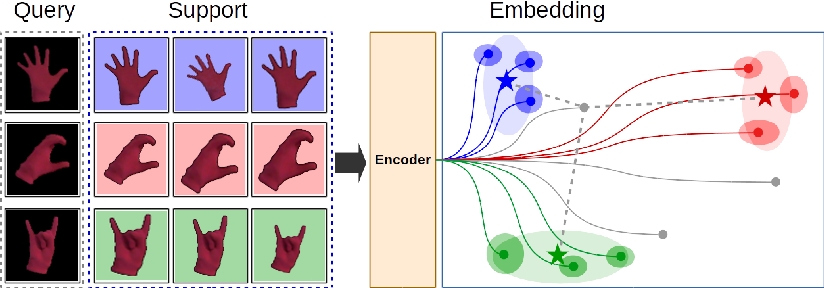
\includegraphics[width=1.0\columnwidth]{images/background/protonets.png}}
    \caption{Prototypical Networks given a set of query samples and support set}
    \label{fig:protonet:handshape}
\end{figure}

Prototypical Networks apply an inductive bias in the form of class prototypes to achieve impressive few-shot performance. The key assumption is the existence of an embedding in which samples from each class cluster around a single prototypical representation which is simply the mean of the individual samples. This idea streamlines n-shot classification in the case of $n > 1$ as classification is simply selecting the label of the closest class prototype, see figure \ref{fig:protonet}.

Schemes for few shot classification tasks like Prototypical Networks can also be of use for training small datasets.

\begin{figure}[!ht]
    \centerline{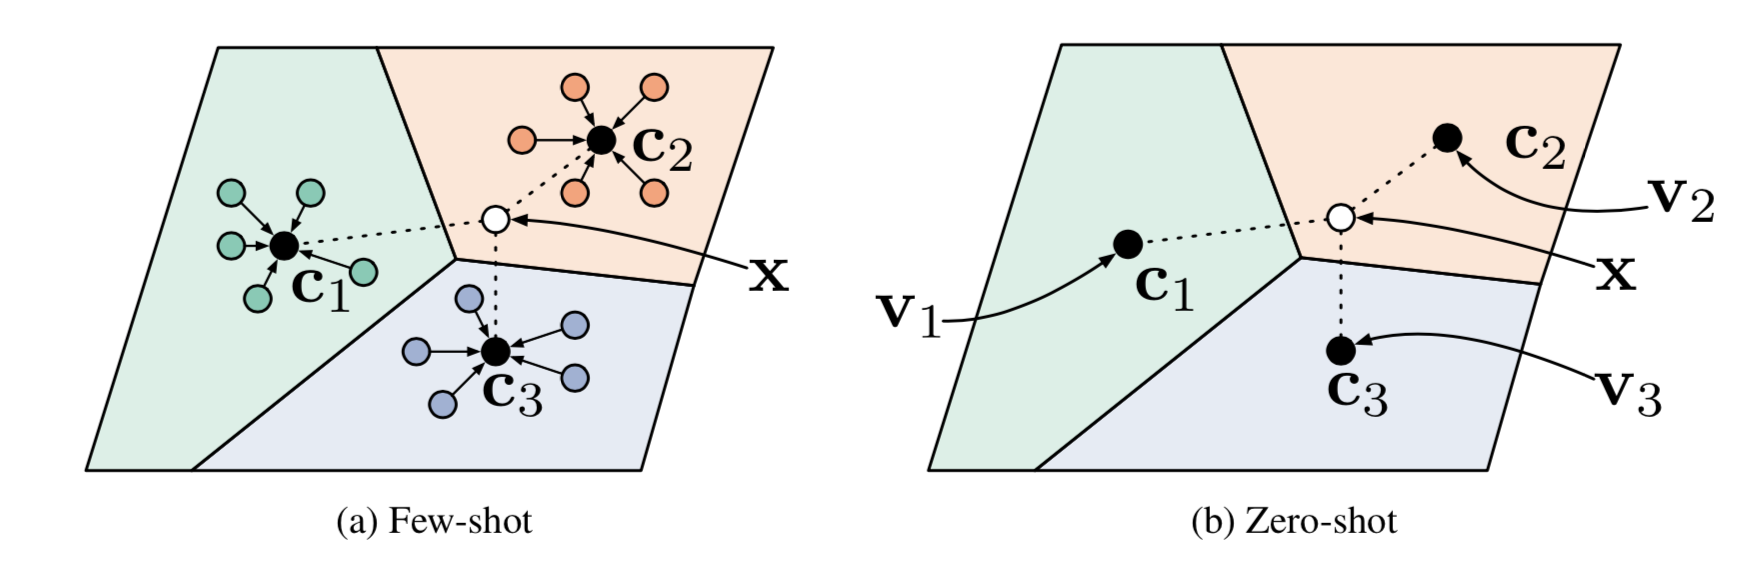
\includegraphics[width=1.15\columnwidth]{images/background/prototypical-networks.png}}
    \caption{Prototypical networks in the few-shot and zero-shot scenarios. \textbf{Left}: Few-shot prototypes
    $\mathbf{c}_k$ are computed as the mean of embedded support examples for each class. \textbf{Right}: Zero-shot prototypes $\mathbf{c}_k$ are produced by embedding class meta-data $\mathbf{v}_k$. In either case, embedded query points are classified via a softmax over distances to class prototypes.}
    \label{fig:protonet}
\end{figure}


\section{Experiments}
\label{sec:experiments}
We performed experiments with the models described in section \ref{sec:models}.

We performed classification experiments on LSA16, RWTH and CIARP handshape datasets. We used $k$-fold cross-validation \cite{Refaeilzadeh2009} randomly partitioning the original dataset into $k = 5$ equal sized subsamples.

For each subsample, we split the dataset in training and test sets, with the latter taking 25\% of the samples. The used splits were stratified, maintaining the proportion of samples of each class in both sets. At the same time, we define validation subsets for each training process. The sets are created with a number of samples per class of 20\% of the number of samples per class of the train set used in each scenario.

We performed experiments using the embedding architectures and configurations described in the following subsections varying the training sample sizes taking 5, 10, 15 and 20 samples, adding the scenarios of 30, 40 and 100 samples per class for CIARP and 30 and 40 for RWTH since they have a bigger amount of samples. In the case of RWTH, those classes that do not have at least 40 samples to carry out the training are filtered.

The same data augmentation was used for each experiment, with which the best results were obtained in previous works \cite{cornejo2019hand}. We applied normalization feature-wise subtracting the mean and dividing by the standard deviation of each feature. For data augmentation we used horizontal flipping,  random rotations from $0\deg$ to $10\deg$ and random resampling. The resampling is performed by reducing each image by 10\% or 20\% in width and height.

\subsection{Wide-DenseNet} \label{sec:experiments:densenet}

\subsubsection{Metodology}

Based on the results obtained in previous works \cite{cornejo2019hand}, we use DenseNet in the following way. We include SE blocks after each dense and transition block. We trained the models using a batch size of 32, an initial learning rate of $10^{-3}$ and 200 epochs with a maximum patience of 55. The resulting model used a growth rate of 64 and two dense blocks with 6 and 12 layers respectively, for all datasets.

\subsubsection{Results}

In tables \ref{tab:results:ciarp:densenet}, \ref{tab:results:lsa16:densenet} and \ref{tab:results:rwth:densenet} we can see the results obtained using Wide-Densenet on CIARP, LSA16 and RWTH, respectively. We can notice the low accuracy obtained in the subsets of 5 samples and how the accuracy increases when the number of samples is bigger.

The following sections compare the results obtained for each experiment with those obtained by Wide-DenseNet.

\doublerulesep 0.1pt
\begin{table*}[!ht]
\begin{footnotesize}
\caption{Accuracy obtained by Wide-DenseNet on CIARP as number of training samples is varied.} \label{tab:results:ciarp:densenet}
\makebox[1 \textwidth][c]{
\centering
\begin{tabular}{ p{8em} p{6em} p{6em} p{6em} p{6em} p{6em} p{6em} p{6em} p{6em} }
\toprule
\emph{Method} & \emph{5 samples} & \emph{10 samples} &  \emph{15 samples} & \emph{20 samples} & \emph{30 samples} & \emph{40 samples} & \emph{100 samples} & \emph{360 samples} \\ \midrule

DenseNet           &   10.00 $\pm$ 0.00  &   10.00 $\pm$ 0.00  &   37.26 $\pm$ 36.81 &   76.07 $\pm$ 37.87 &   82.71 $\pm$ 38.35 &   99.83 $\pm$ 0.28  &   99.95 $\pm$ 0.04  &   99.83 $\pm$ 0.24  \\

\bottomrule
\end{tabular}
} %close centering
\end{footnotesize}
\end{table*}


\doublerulesep 0.1pt
\begin{table*}[!ht]
\begin{footnotesize}
\caption{Accuracy of Wide-DenseNet on LSA16 as number of training samples is varied.} \label{tab:results:lsa16:densenet}
\makebox[1 \textwidth][c]{
\centering
\begin{tabular}{ p{9em} p{7em} p{7em} p{7em} p{7em} p{7em} }
\toprule
\emph{Method} & \emph{5 samples} & \emph{10 samples} &  \emph{15 samples} & \emph{20 samples} & \emph{30 samples}   \\ \midrule

DenseNet           &    6.56 $\pm$ 0.63  &   92.80 $\pm$ 2.89  &   92.81 $\pm$ 2.82  &   95.31 $\pm$ 1.23  &   96.13 $\pm$ 0.00   \\

\bottomrule
\end{tabular}
} %close centering
\end{footnotesize}
\end{table*}


\doublerulesep 0.1pt
\begin{table*}[!ht]
\begin{footnotesize}
\caption{Accuracy of Wide-DenseNet on RWTH as number of training samples is varied.} \label{tab:results:rwth:densenet}
\makebox[1 \textwidth][c]{
\centering
\begin{tabular}{ p{9em} p{7em} p{7em} p{7em} p{7em} p{7em} p{7em} p{7em} }
\toprule
\emph{Method}   & \emph{5 samples}    & \emph{10 samples}   &  \emph{15 samples}  & \emph{20 samples}   & \emph{30 samples}   & \emph{40 samples}   & \emph{Full RWTH} \\ \midrule

DenseNet           &   10.32 $\pm$ 2.48  &   17.78 $\pm$ 17.08 &   46.66 $\pm$ 19.17 &   64.59 $\pm$ 3.81  &   71.20 $\pm$ 2.24  &   71.85 $\pm$ 3.84  &   96.05 $\pm$ 0.96 \\

\bottomrule
\end{tabular}
} %close centering
\end{footnotesize}
\end{table*}

\subsection{Transfer Learning} \label{sec:experiments:tl}

\subsubsection{Metodology}

We performed experiments in every dataset to figure out which Transfer Learning configuration is more convenient. For each dataset, experiments are carried out varying the dataset on which the base model used to define the embedding architecture is trained. With this approach, it is possible to define an experiment matrix seeking to evaluate which dataset is the best option when transferring learning over another.

Our embedding architecture consists of a sequential model with a pretrained DenseNet model, global average pooling, a hidden dense layer with a ReLU nonlinearity and finally a softmax classifier. Since CIARP contains only gray scale images, an input layer and a 3x3 convolutional layer are prepended to the sequential model.

Furthermore, in this set of experiments CIFAR10\cite{cifar10dataset} and MNIST\cite{lecun-mnisthandwrittendigit-2010} are added to the datasets which are used for the construction of the pre-trained models.

\subsubsection{Results}

In tables \ref{tab:results:ciarp:tl}, \ref{tab:results:lsa16:tl} and \ref{tab:results:rwth:tl} we can see the results obtained using models trained with Transfer Learning on CIARP, LSA16 and RWTH, respectively. We can notice the low accuracy obtained in the subsets of 5 samples and how the accuracy increases when the number of samples is bigger.

In the case of CIARP, the use of transfer learning gives significantly better results than those obtained by Wide-DenseNet for those cases in which the number of training examples is less than 40, therefore the use of this method is advantageous. Considering this and the results obtained in LSA16, the use of Transfer Learning on those datasets means an advantage over the accuracy obtained by Wide-DenseNet model, however it is not so in the case of RWTH.

\doublerulesep 0.1pt
\begin{table*}[!ht]
\begin{footnotesize}
\caption{Accuracy of various models trained using Transfer Learning on CIARP compared to the accuracy obtained by Wide-DenseNet. Each method named as \textit{TL + D} represents a transfer learning method using a model pretrained in \textit{D} dataset.} \label{tab:results:ciarp:tl}
\makebox[1 \textwidth][c]{
\centering
\begin{tabular}{ p{8em} p{6em} p{6em} p{6em} p{6em} p{6em} p{6em} p{6em} p{6em} }
\toprule
\emph{Method} & \emph{5 samples} & \emph{10 samples} &  \emph{15 samples} & \emph{20 samples} & \emph{30 samples} & \emph{40 samples} & \emph{100 samples} & \emph{360 samples} \\ \midrule

DenseNet      &   10.00 $\pm$ 0.00  &   10.00 $\pm$ 0.00  &   37.26 $\pm$ 36.81 &   76.07 $\pm$ 37.87 &   82.71 $\pm$ 38.35 &   99.73 $\pm$ 0.28  &   99.95 $\pm$ 0.04  &   \textbf{99.83 $\pm$ 0.24}  \\
TL + CIFAR10  &   \textbf{11.69 $\pm$ 3.39}  &   \textbf{27.24 $\pm$ 33.54} &   98.44 $\pm$ 0.47  &   98.71 $\pm$ 0.72  &   \textbf{99.61 $\pm$ 0.21}  &   99.64 $\pm$ 0.31  &   99.92 $\pm$ 0.05  &   99.59 $\pm$ 0.19  \\
TL + MNIST    &   10.00 $\pm$ 0.00  &   10.00 $\pm$ 0.00  &   97.31 $\pm$ 1.36  &   \textbf{99.25 $\pm$ 0.37}  &   99.30 $\pm$ 0.48  &   99.70 $\pm$ 0.31  &   \textbf{99.95 $\pm$ 0.03}  &   99.21 $\pm$ 0.51  \\
TL + LSA16    &   11.19 $\pm$ 2.38  &   10.01 $\pm$ 0.02  &   97.82 $\pm$ 0.93  &   99.07 $\pm$ 0.45  &   99.51 $\pm$ 0.24  &   99.73 $\pm$ 0.33  &   99.93 $\pm$ 0.06  &   99.73 $\pm$ 0.26  \\
TL + RWTH     &   10.24 $\pm$ 0.49  &   10.03 $\pm$ 0.04  &   \textbf{98.59 $\pm$ 0.83}  &   98.33 $\pm$ 1.16  &   99.58 $\pm$ 0.20  &   \textbf{99.74 $\pm$ 0.16}  &   99.85 $\pm$ 0.09  &   99.42 $\pm$ 0.40  \\

\bottomrule
\end{tabular}
} %close centering
\end{footnotesize}
\end{table*}


\doublerulesep 0.1pt
\begin{table*}[!ht]
\begin{footnotesize}
\caption{Accuracy of various models trained using Transfer Learning on LSA16 compared to the accuracy obtained by Wide-DenseNet. Each method named as \textit{TL + D} represents a transfer learning method using a model pretrained in \textit{D} dataset.} \label{tab:results:lsa16:tl}
\makebox[1 \textwidth][c]{
\centering
\begin{tabular}{ p{9em} p{7em} p{7em} p{7em} p{7em} p{7em} }
\toprule
\emph{Method} & \emph{5 samples} & \emph{10 samples} &  \emph{15 samples} & \emph{20 samples} & \emph{30 samples}   \\ \midrule

DenseNet           &    6.56 $\pm$ 0.63  &   92.80 $\pm$ 2.89  &   92.81 $\pm$ 2.82  &   95.31 $\pm$ 1.23  &   96.13 $\pm$ 0.00   \\
TL + CIFAR10       &    6.25 $\pm$ 0.00  &   \textbf{92.91 $\pm$ 2.66}  &   \textbf{93.75 $\pm$ 2.30}  &   94.79 $\pm$ 1.14  &   \textbf{97.91 $\pm$ 0.46}   \\
TL + MNIST         &    6.25 $\pm$ 0.00  &   92.60 $\pm$ 2.07  &   93.43 $\pm$ 1.73  &   95.41 $\pm$ 2.42  &   97.08 $\pm$ 0.62   \\
TL + CIARP         &    6.25 $\pm$ 0.00  &   92.70 $\pm$ 1.77  &   92.60 $\pm$ 1.87  &   \textbf{96.67 $\pm$ 1.12}  &   96.24 $\pm$ 1.48   \\
TL + RWTH          &    \textbf{6.97 $\pm$ 1.45}  &   74.79 $\pm$ 34.27 &   93.43 $\pm$ 2.56  &   95.62 $\pm$ 1.21  &   96.97 $\pm$ 0.89   \\

\bottomrule
\end{tabular}
} %close centering
\end{footnotesize}
\end{table*}


\doublerulesep 0.1pt
\begin{table*}[!ht]
\begin{footnotesize}
\caption{Accuracy of various models trained using Transfer Learning on RWTH compared to the accuracy obtained by Wide-DenseNet. Each method named as \textit{TL + D} represents a transfer learning method using a model pretrained in \textit{D} dataset.} \label{tab:results:rwth:tl}
\makebox[1 \textwidth][c]{
\centering
\begin{tabular}{ p{9em} p{7em} p{7em} p{7em} p{7em} p{7em} p{7em} p{7em} }
\toprule
\emph{Method}   & \emph{5 samples}    & \emph{10 samples}   &  \emph{15 samples}  & \emph{20 samples}   & \emph{30 samples}   & \emph{40 samples}   & \emph{Full RWTH} \\ \midrule

DenseNet        &   10.32 $\pm$ 2.48  &   17.78 $\pm$ 17.08 &   \textbf{46.66 $\pm$ 19.17} &   \textbf{64.59 $\pm$ 3.81}  &   \textbf{71.20 $\pm$ 2.24}  &   \textbf{71.85 $\pm$ 3.84}  &   \textbf{96.05 $\pm$ 0.96} \\
TL + CIFAR10    &   \textbf{10.73 $\pm$ 1.59}  &   17.78 $\pm$ 17.21 &   18.25 $\pm$ 16.33 &   48.19 $\pm$ 21.08 &   65.76 $\pm$ 6.50  &   66.28 $\pm$ 4.67  &   95.29 $\pm$ 1.22   \\
TL + MNIST      &    9.89 $\pm$ 1.49  &   17.32 $\pm$ 15.89 &   21.12 $\pm$ 18.70 &   37.13 $\pm$ 24.93 &   64.91 $\pm$ 3.54  &   63.66 $\pm$ 3.86  &   96.16 $\pm$ 0.58   \\
TL + CIARP      &    9.31 $\pm$ 1.90  &   \textbf{18.30 $\pm$ 16.49} &   25.79 $\pm$ 21.30 &   39.07 $\pm$ 24.93 &   64.26 $\pm$ 5.42  &   66.69 $\pm$ 3.15  &   95.57 $\pm$ 1.06   \\
TL + LSA16      &    8.33 $\pm$ 0.00  &   17.15 $\pm$ 15.69 &   28.93 $\pm$ 24.06 &   46.22 $\pm$ 20.08 &   66.58 $\pm$ 5.00  &   62.89 $\pm$ 10.14 &   95.48 $\pm$ 0.30  \\

\bottomrule
\end{tabular}
} %close centering
\end{footnotesize}
\end{table*}

\subsection{Model-Agnostic Meta-Learning}

\subsubsection{Metodology}

We employed the Wide-DenseNet architecture explained before \ref{sec:experiments:densenet} applying the Model-Agnostic Meta-Learning technique to the training process. In the work of Finn et al. \cite{DBLP:journals/corr/FinnAL17} they follow the experimental protocol proposed by Vinyals et al. \cite{DBLP:journals/corr/VinyalsBLKW16}, which involves fast learning of N-way classification with 1 or 5 shots. This is the protocol that we used for Prototypical Networks but not for the set of experiments that we propose in this section.

In this case, we test the performance of MAML applied to training scenarios similar to those used with Wide-DenseNet in the experiments described in section \ref{sec:experiments:densenet}, so the training process will work with batches in the following way. We trained a Wide-DenseNet model using the MAML technique over one task before doing the meta-learning. That task will correspond to short training process on a \textit{D} dataset following the process described in section \ref{sec:models:maml} . Then we use the trained model to initialize the weights for a new model. The new model is treated as a new task. Our model was trained on one task and we used this previous knowledge to initialize the weights of the model for a new task, using a training process similar to the used for the experiments we performed using Transfer Learning described in section \ref{sec:experiments:tl}.

\subsubsection{Results}

In tables \ref{tab:results:ciarp:maml}, \ref{tab:results:lsa16:maml} and \ref{tab:results:rwth:maml} we can see the results obtained using models trained with MAML technique on CIARP, LSA16 and RWTH, respectively. Again, we can see the low accuracy obtained in the subsets of 5 samples and how the accuracy increases when the number of samples is bigger.

In the case of CIARP, the use of MAML gives significantly better results than those obtained by Wide-DenseNet for those cases in which the number of training examples is less than 40, therefore the use of this method is advantageous. Considering this and the results obtained in LSA16, the use of Transfer Learning on those datasets means an advantage over the accuracy obtained by Wide-DenseNet model, however it is not so in the case of RWTH. \\

\doublerulesep 0.1pt
\begin{table*}[!ht]
\begin{footnotesize}
\caption{Accuracy of various models trained using Model-Agnostic Meta-Learning on CIARP compared to the accuracy obtained by Wide-DenseNet. Each method named as \textit{MAML + D} represents a MAML method using a model pretrained in \textit{D} dataset.} \label{tab:results:ciarp:maml}
\makebox[1 \textwidth][c]{
\centering
\begin{tabular}{ p{8em} p{6em} p{6em} p{6em} p{6em} p{6em} p{6em} p{6em} p{6em} }
\toprule
\emph{Method} & \emph{5 samples} & \emph{10 samples} &  \emph{15 samples} & \emph{20 samples} & \emph{30 samples} & \emph{40 samples} & \emph{100 samples} & \emph{360 samples} \\ \midrule

DenseNet           &   10.00 $\pm$ 0.00  &   10.00 $\pm$ 0.00  &   37.26 $\pm$ 36.81 &   76.07 $\pm$ 37.87 &   82.71 $\pm$ 38.35 &   99.83 $\pm$ 0.28  &   99.95 $\pm$ 0.04  &   \textbf{99.83 $\pm$ 0.24}  \\
MAML               &   11.12 $\pm$ 2.24  &   \textbf{26.53 $\pm$ 33.07} &   80.23 $\pm$ 35.13 &   98.85 $\pm$ 0.99  &   99.71 $\pm$ 0.15  &   99.56 $\pm$ 0.34  &   99.94 $\pm$ 0.04  &   99.01 $\pm$ 0.66  \\
MAML + CIFAR10     &   10.47 $\pm$ 0.94  &   10.00 $\pm$ 0.00  &   95.51 $\pm$ 2.15  &   98.41 $\pm$ 1.16  &   \textbf{99.73 $\pm$ 0.30}  &   98.92 $\pm$ 1.72  &   99.96 $\pm$ 0.02  &   99.44 $\pm$ 0.38  \\
MAML + MNIST       &   10.00 $\pm$ 0.00  &   12.70 $\pm$ 3.27  &   80.13 $\pm$ 35.07 &   98.91 $\pm$ 0.47  &   99.64 $\pm$ 0.16  &   \textbf{99.74 $\pm$ 0.16}  &   99.97 $\pm$ 0.04  &   99.43 $\pm$ 0.64  \\
MAML + LSA16       &   \textbf{11.38 $\pm$ 2.65}  &   11.44 $\pm$ 2.49  &   80.10 $\pm$ 35.07 &   98.95 $\pm$ 0.64  &   99.51 $\pm$ 0.45  &   99.50 $\pm$ 0.62  &   99.93 $\pm$ 0.08  &   99.30 $\pm$ 0.61  \\
MAML + RWTH        &   10.00 $\pm$ 0.00  &   10.00 $\pm$ 0.00  &   \textbf{97.75 $\pm$ 0.52}  &   \textbf{99.07 $\pm$ 0.63}  &   99.64 $\pm$ 0.18  &   99.65 $\pm$ 0.17  &   \textbf{99.97 $\pm$ 0.02}  &   99.08 $\pm$ 0.73  \\

\bottomrule
\end{tabular}
} %close centering
\end{footnotesize}
\end{table*}

\doublerulesep 0.1pt
\begin{table*}[!ht]
\begin{footnotesize}
\caption{Accuracy of various models trained using Model-Agnostic Meta-Learning on LSA16 compared to the accuracy obtained by Wide-DenseNet. Each method named as \textit{MAML + D} represents a MAML method using a model pretrained in \textit{D} dataset.} \label{tab:results:lsa16:maml}
\makebox[1 \textwidth][c]{
\centering
\begin{tabular}{ p{9em} p{7em} p{7em} p{7em} p{7em} p{7em} }
\toprule
\emph{Method} & \emph{5 samples} & \emph{10 samples} &  \emph{15 samples} & \emph{20 samples} & \emph{30 samples}   \\ \midrule

DenseNet           &    6.56 $\pm$ 0.63  &   92.80 $\pm$ 2.89  &   92.81 $\pm$ 2.82  &   95.31 $\pm$ 1.23  &   96.13 $\pm$ 0.00   \\
MAML               &    6.35 $\pm$ 0.20  &   \textbf{93.95 $\pm$ 1.53}  &   93.54 $\pm$ 1.60  &   95.72 $\pm$ 1.00  &   \textbf{97.81 $\pm$ 0.38}   \\
MAML + CIFAR10     &    6.25 $\pm$ 0.00  &   92.18 $\pm$ 1.47  &   94.06 $\pm$ 1.76  &   95.63 $\pm$ 2.60  &   97.08 $\pm$ 0.77   \\
MAML + MNIST       &    6.45 $\pm$ 0.41  &   92.91 $\pm$ 0.96  &   94.17 $\pm$ 2.45  &   95.63 $\pm$ 1.16  &   97.18 $\pm$ 0.41   \\
MAML + CIARP       &    6.77 $\pm$ 0.65  &   92.08 $\pm$ 2.51  &   \textbf{94.58 $\pm$ 1.16}  &   \textbf{96.14 $\pm$ 1.34}  &   96.97 $\pm$ 1.25   \\
MAML + RWTH        &    \textbf{6.87 $\pm$ 0.76}  &   92.81 $\pm$ 0.51  &   94.47 $\pm$ 2.29  &   94.37 $\pm$ 2.58  &   96.24 $\pm$ 1.00   \\

\bottomrule
\end{tabular}
} %close centering
\end{footnotesize}
\end{table*}

\doublerulesep 0.1pt
\begin{table*}[!ht]
\begin{footnotesize}
\caption{Accuracy of various models trained using Model-Agnostic Meta-Learning on RWTH compared to the accuracy obtained by Wide-DenseNet. Each method named as \textit{MAML + D} represents a MAML method using a model pretrained in \textit{D} dataset.} \label{tab:results:rwth:maml}
\makebox[1 \textwidth][c]{
\centering
\begin{tabular}{ p{9em} p{7em} p{7em} p{7em} p{7em} p{7em} p{7em} p{7em} }
\toprule
\emph{Method}   & \emph{5 samples}    & \emph{10 samples}   &  \emph{15 samples}  & \emph{20 samples}   & \emph{30 samples}   & \emph{40 samples}   & \emph{Full RWTH} \\ \midrule

DenseNet           &   10.32 $\pm$ 2.48  &   \textbf{17.78 $\pm$ 17.08} &   \textbf{46.66 $\pm$ 19.17} &   \textbf{64.59 $\pm$ 3.81}  &   \textbf{71.20 $\pm$ 2.24}  &   \textbf{71.85 $\pm$ 3.84}  &   \textbf{96.05 $\pm$ 0.96} \\
MAML               &    9.20 $\pm$ 1.97  &    9.86 $\pm$ 1.29  &   25.38 $\pm$ 19.31 &   30.51 $\pm$ 24.03 &   67.81 $\pm$ 1.99  &   67.13 $\pm$ 1.55  &   95.54 $\pm$ 1.21   \\
MAML + CIFAR10     &    8.36 $\pm$ 0.62  &    9.69 $\pm$ 1.94  &    8.66 $\pm$ 1.75  &   38.90 $\pm$ 24.40 &   64.56 $\pm$ 7.86  &   64.53 $\pm$ 3.18  &   96.08 $\pm$ 0.37   \\
MAML + MNIST       &    9.80 $\pm$ 1.27  &    9.80 $\pm$ 2.03  &   28.33 $\pm$ 21.66 &   51.12 $\pm$ 21.42 &   66.93 $\pm$ 3.13  &   69.07 $\pm$ 4.66  &   95.73 $\pm$ 0.56   \\
MAML + CIARP       &    9.83 $\pm$ 2.80  &   17.59 $\pm$ 16.62 &   19.15 $\pm$ 18.97 &   38.57 $\pm$ 23.35 &   66.50 $\pm$ 3.05  &   66.36 $\pm$ 3.02  &   96.00 $\pm$ 0.35   \\
MAML + LSA16       &   \textbf{10.98 $\pm$ 3.66}  &   15.16 $\pm$ 11.85 &   28.57 $\pm$ 23.10 &   46.96 $\pm$ 19.03 &   67.18 $\pm$ 4.49  &   64.42 $\pm$ 3.58  &   95.48 $\pm$ 1.29   \\

\bottomrule
\end{tabular}
} %close centering
\end{footnotesize}
\end{table*}

\subsection{Prototypical Network}

As mentioned in section \ref{models:protonet}, we can use Prototypical Networks' ability to work with small datasets even if all samples are labeled. Based on the results obtained in previous works \cite{cornejo2019hand}, we use Prototypical Networks with the following configuration.

\subsubsection{Metodology}

Our Prototypical Networks employ an embedding architecture composed of four convolutional blocks. Each block comprises a 64-filter $3 \times 3$ convolution, followed by a batch normalization layer, a ReLU nonlinearity and $2 x 2$ max-pooling.

We used the same encoder for embedding both support and query points. All of our models were trained with the ADAM\cite{Adam} optimizer. We used an initial learning rate of $10^{-3}$ and cut the learning rate in half every $2000$ episodes.

We trained the networks using Euclidean distance in the 1-shot and 5-shot scenarios with training episodes containing 16, 20 and 10 classes (for LSA16, RWTH and CIARP respectively) and 5 query points per class when possible. We computed classification accuracy for our models by averaging over 1000 randomly generated episodes from the test set.

In previous works \cite{cornejo2019hand}, we found that the difference in the results obtained in 1-shot and 5-shot scenarios for these datasets was very large. On the other hand, 5-shot scenarios gave better results. Therefore, we only used 1-shot learning in the experiments in which the minimum number of examples per class does not allow to use 5-shot.

\subsubsection{Results}

In tables \ref{tab:results:ciarp:proto}, \ref{tab:results:lsa16:proto} and \ref{tab:results:rwth:proto} we can see the results obtained using models trained with MAML technique on CIARP, LSA16 and RWTH, respectively. 

Prototypical Networks have similar accuracy for LSA16 and CIARP datasets beating the Wide-DenseNet models for the 5 and 10 samples scenarios, and also the other splits in the case of LSA16. In the case of CIARP, although it did not obtain the best results for all subsets, it achieved a very good performance in all cases, and similar results for the obtained by Wide-DenseNet.

Regarding RWTH, we can notice that Prototypical Networks cannot take advantage of the images and the accuracy does not increase as the number of samples do. It is possible that Prototypical Networks obtained the lowest accuracy because the images of the hands were unsegmented. In this case, the accuracy of Wide-DenseNet is slightly bigger than Prototypical Networks model when the number of samples per class, N, is bigger than 15.

\doublerulesep 0.1pt
\begin{table*}[!ht]
\begin{footnotesize}
\caption{Accuracy of Prototypical Networks based model on CIARP compared to the accuracy obtained by Wide-DenseNet.} \label{tab:results:ciarp:proto}
\makebox[1 \textwidth][c]{
\centering
\begin{tabular}{ p{8em} p{6em} p{6em} p{6em} p{6em} p{6em} p{6em} p{6em} p{6em} }
\toprule
\emph{Method} & \emph{5 samples} & \emph{10 samples} &  \emph{15 samples} & \emph{20 samples} & \emph{30 samples} & \emph{40 samples} & \emph{100 samples} & \emph{360 samples} \\ \midrule

DenseNet           &   10.00 $\pm$ 0.00  &   10.00 $\pm$ 0.00  &   37.26 $\pm$ 36.81 &   76.07 $\pm$ 37.87 &   82.71 $\pm$ 38.35 &   99.83 $\pm$ 0.28  &   \textbf{99.95 $\pm$ 0.04}  &   \textbf{99.83 $\pm$ 0.24}  \\
ProtoNet           &   \textbf{91.45 $\pm$ 2.44}  &   \textbf{94.48 $\pm$ 1.78}  &   \textbf{95.70 $\pm$ 0.66}  &   \textbf{97.63 $\pm$ 0.68}  &   \textbf{98.38 $\pm$ 0.27}  &   \textbf{99.21 $\pm$ 0.28}  &   99.82 $\pm$ 0.05  &   99.41 $\pm$ 0.16  \\

\bottomrule
\end{tabular}
} %close centering
\end{footnotesize}
\end{table*}

\doublerulesep 0.1pt
\begin{table*}[!ht]
\begin{footnotesize}
\caption{Accuracy of Prototypical Networks based model on LSA16 compared to the accuracy obtained by Wide-DenseNet.} \label{tab:results:lsa16:proto}
\makebox[1 \textwidth][c]{
\centering
\begin{tabular}{ p{9em} p{7em} p{7em} p{7em} p{7em} p{7em} }
\toprule
\emph{Method} & \emph{5 samples} & \emph{10 samples} &  \emph{15 samples} & \emph{20 samples} & \emph{30 samples}   \\ \midrule

DenseNet           &    6.56 $\pm$ 0.63  &   92.80 $\pm$ 2.89  &   92.81 $\pm$ 2.82  &   95.31 $\pm$ 1.23  &   96.13 $\pm$ 0.00   \\
ProtoNet           &   \textbf{94.15 $\pm$ 1.27}  &   \textbf{94.64 $\pm$ 1.23}  &   \textbf{95.50 $\pm$ 1.01}  &   \textbf{97.20 $\pm$ 0.74}  &   \textbf{98.38 $\pm$ 0.22}   \\

\bottomrule
\end{tabular}
} %close centering
\end{footnotesize}
\end{table*}

\doublerulesep 0.1pt
\begin{table*}[!ht]
\begin{footnotesize}
\caption{Accuracy of Prototypical Networks based model on RWTH compared to the accuracy obtained by Wide-DenseNet.} \label{tab:results:rwth:proto}
\makebox[1 \textwidth][c]{
\centering
\begin{tabular}{ p{9em} p{7em} p{7em} p{7em} p{7em} p{7em} p{7em} p{7em} }
\toprule
\emph{Method}   & \emph{5 samples}    & \emph{10 samples}   &  \emph{15 samples}  & \emph{20 samples}   & \emph{30 samples}   & \emph{40 samples}   & \emph{Full RWTH} \\ \midrule

DenseNet           &   10.32 $\pm$ 2.48  &   17.78 $\pm$ 17.08 &   46.66 $\pm$ 19.17 &   \textbf{64.59 $\pm$ 3.81}  &   \textbf{71.20 $\pm$ 2.24}  &   \textbf{71.85 $\pm$ 3.84}  &   \textbf{96.05 $\pm$ 0.96} \\
ProtoNet           &   \textbf{48.93 $\pm$ 3.02}  &   \textbf{48.53 $\pm$ 1.59}  &   \textbf{48.87 $\pm$ 1.60}  &   46.73 $\pm$ 1.14  &   47.58 $\pm$ 1.33  &   50.36 $\pm$ 6.82  &   47.09 $\pm$ 0.10   \\

\bottomrule
\end{tabular}
} %close centering
\end{footnotesize}
\end{table*}



\subsection{Discussion}
\label{sec:results}
Figure \ref{fig:results_varying_samples} shows the accuracy of the different models for various training set sizes, as explained in section \ref{sec:experiments}. Each subset corresponds to a tick in the x axis named \textit{N} which is the number of samples per class for the training split. 

The results of the experiments using MAML and Transfer Learning are grouped according to the dataset with which the pretrained DenseNet model was created.

Prototypical Networks have similar accuracy for LSA16 and CIARP datasets beating the rest of the models for the 5 and 10 samples scenarios, and also the other splits in the case of LSA16. In the case of CIARP, although it did not obtain the best results for all subsets, it achieved a very good performance in all cases, and similar results for the rest of the models.

Regarding RWTH, we can notice that Prototypical Networks cannot take advantage of the images and the accuracy does not increase as the number of samples do. It is possible that Prototypical Networks obtained the lowest accuracy because the images of the hands were unsegmented. In this case, the accuracy of DenseNet is slightly bigger than for other when the number of samples per class, N, is bigger than 15.

On the other hand, we can observe the low accuracy obtained in most experiments that use DenseNet in the subset of 5 samples.

The use of MAML in DenseNet training increses its accuracy in LSA16 and CIARP. However, the use of MAML and Transfer Learning does not bring advantages in the accuracy obtained in RWTH compared to that obtained by the DenseNet model used.

From the obtained results, we can see that the performance of the DenseNet based models increases as more training examples are provided. The use of MAML and Transfer Learning on CIARP and LSA16 means an advantage over the accuracy obtained by the DenseNet model, however it is not so in the case of RWTH. On the other hand, Prototypical Networks models do not show a significant increase in performance as the number of samples increases, always being a good choice with few samples where the hands are segmented.

\begin{figure*}[!ht]
\centering
\begin{tabular}{c}
    \subfigure[Accuracy of Prototypical Networks and DenseNet models trained by varying sample sizes on CIARP taking the results for less than 100 samples.]{
        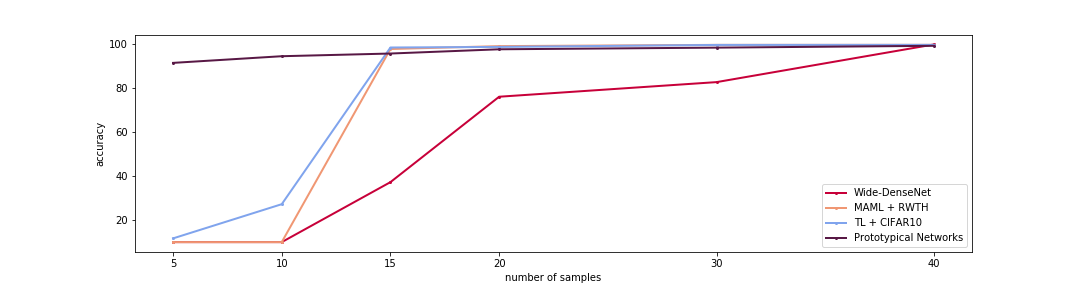
\includegraphics[width=1\textwidth]{results/ciarp.png}
    } \\
    \subfigure[Accuracy of Prototypical Networks and DenseNet models trained by varying sample sizes on LSA16.]{
        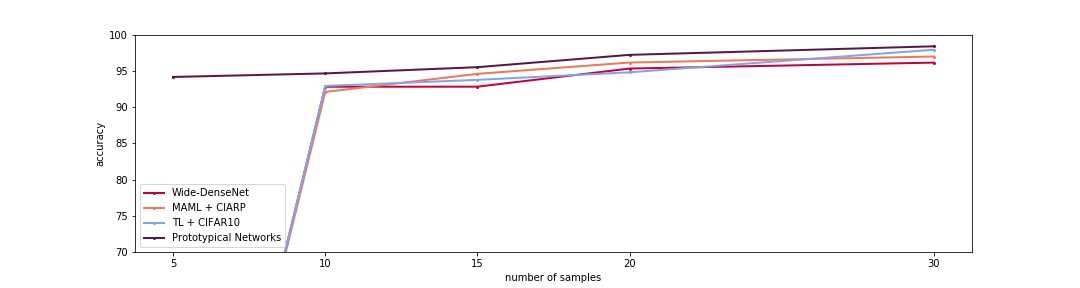
\includegraphics[width=1\textwidth]{results/lsa16.png}
    } \\
    \subfigure[Accuracy of Prototypical Networks and DenseNet models trained by varying sample sizes on LSA16.]{
        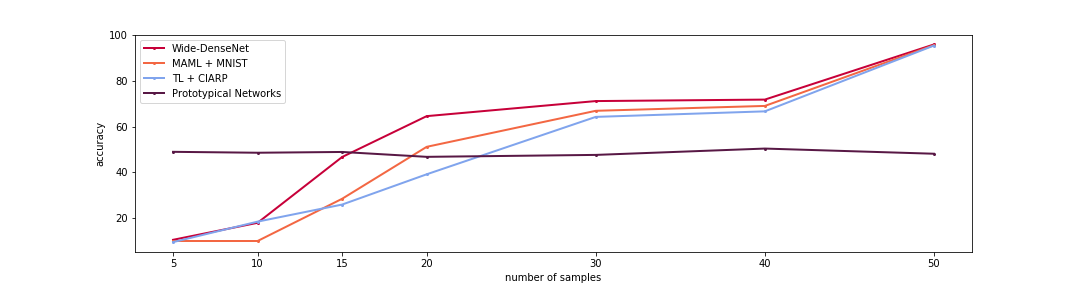
\includegraphics[width=1\textwidth]{results/rwth.png}
    } \\
\end{tabular}
\caption{Accuracy of various models on datasets CIARP, LSA16 and RWTH, respectively. Each plot represents a different dataset, and each line a model that corresponds to the best results obtained on every technique described en section \ref{sec:experiments}. The x-axis indicates the number of samples used to train the model and the y-axis its accuracy. \label{fig:results_varying_samples}}
\end{figure*}


\section{Conclusion}
\label{sec:conclusion}
We have performed experiments to evaluate the accuracy of Prototypical Networks, Wide-DenseNet, MAML and Transfer Learning on three handshape recognition datasets. For all datasets we found models that showed a performance on par with or better than the state of the art. All models achieve near-perfect accuracy on CIARP. This shows that the dataset is too simple as a benchmark for handshape recognition. While it has more samples than the other datasets (6000), they are too homogeneous and do not have enough variation.

In  future  work,  we  will  focus  on  comparing  with  other  datasets  to  better understand the relationship between models and dataset complexities for hand-shape  recognition.  We  also  see  the  need to  compare with the use of MAML models pretrained with different tasks, combining datasets to achieve it. Adding to future plans, we are going to research on methods that can take advantage of unlabeled data and investigate the possibility of merging data sets from different sign languages to augment the sample size, as well as identify the types of data augmentation that lead to an improvement in state-of-the-art models.


\bibliographystyle{unsrt}
\bibliography{references,related}

\end{document}
